\documentclass[12pt]{article}
\usepackage{multirow}
\usepackage{graphicx}
\usepackage{times}
\usepackage[top=4cm,bottom=2cm,left=2cm,right=2cm]{geometry}
\parskip 6pt
\parindent 0pt
\usepackage{tweaklist}
\renewcommand{\itemhook}{\setlength{\topsep}{0pt} \setlength{\itemsep}{0pt}}
\renewcommand{\descripthook}{\setlength{\topsep}{0pt} \setlength{\itemsep}{0pt}}
\renewcommand{\enumhook}{\setlength{\topsep}{0pt} \setlength{\itemsep}{0pt}}

\title{Brontes Frame Grabber Design}
\author{Daniel Drake}
\date{\today}
\begin{document}
\maketitle

\section{Introduction}

The Frame Grabber (FG) will replace the costy and inconvenient IEEE1394-based image capture mechanism used in the Lava Chairside Oral Scanner.

The FG will be custom designed as a PCI card, based on a Eureka PCI core. It will use direct memory access (DMA) to save frames into the computer memory.

Although this is an imaging device, the data transferred is arbitrary: the design makes no assumptions on what the data actually is.

This document details a suggested PCI-level interface to the FG.

\section{Overview}

\subsection{Block diagram}

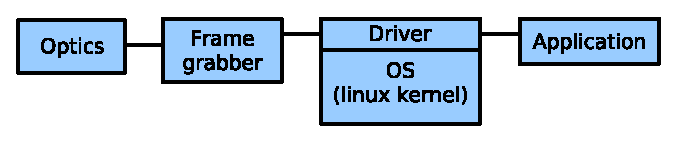
\includegraphics{block.eps}

\subsection{Hardware}

The Eureka EC220 PCI core will be used by the FG. This hardware can act as both a master and target concurrently.

The bus master functionality will be used to write directly into system RAM, using DMA.

The bus target functionality will be used for the driver to request information (e.g. read registers) from the board. The EC220 forwards these requests to user logic.

The PCI configuration space is handled entirely by the EC220, independantly of the user logic.

\subsection{Software}

This project includes the development of an OS-level driver for the hardware. This will be implemented as a Linux kernel driver.

The driver will handle:
\begin{itemize}
\item Hardware detection
\item Hardware initialization
\item Negotiation of DMA transfers
\item Communication of memory addresses to userspace
\end{itemize}

When triggered, the driver will reserve memory regions for frame transfer and communicate these to the hardware.

The driver will create a character device node, which will support mmap() to map the memory regions into userspace. An ioctl will be provided to determine which areas of the memory regions have data, and poll()/select() will be supported in order to notify userspace when the state of the memory regions changes.

At the driver level, this is a truly zero-copy mechanism: the driver itself does not touch the data, it just communicates the addresses of where the hardware put the image data to userspace.

As the driver will be linked against the Linux kernel, the driver itself must be open source, so we must be careful to exclude all sensitive IP from the driver. This should not be a problem given that the driver is simply transporting addresses of arbitrary lumps of data. The proprietary userspace code which uses the driver to locate the images (and then process them) is not bound to the Linux kernel licensing.

\subsection{Hardware/driver communication}

It is worth clarifying the only ways that the driver and the hardware can communicate.

\begin{description}
\item[DMA] The FG can write data into PC physical memory. This communication is invoked by the FG but the driver is not aware when this happens.
\item[Interrupt] The FG can generate an interrupt, which the driver is immediately made aware of. However, no data is passed with the interrupt.
\item[PCI read] The driver can submit read requests to the FG, which are passed to the user logic. The driver provides an address, then the FG immediately provides some data.
\item[PCI write] The driver can submit write requests to the FG, which are passed to user logic. The driver submits both an address and some data.
\end{description}

With these in mind, the driver-instantiated transfers are fairly easy to design: for reading information (e.g. the frame size), a PCI read to a predetermined address can be submitted. The FG will know that this address corresponds to frame size, and the user logic can return the correct result. For writing information (e.g. programming the addresses where the FG should DMA to), the driver can instantiate a PCI write to a predetermined address, with a physical memory address as data.

The FG-to-driver communication is a little less obvious. The FG can DMA to memory at will, but the driver is unaware of this event. The FG can generate the interrupt signal at will, but cannot pass any data alongside with the signal. The solution here is to combine some of the above: some kind of status register will be created, available to the driver using PCI read, which the driver can use to determine the meaning of the interrupt. A common access pattern will look along the lines of:

\begin{enumerate}
\item Frame triplet is ready at FG hardware
\item FG DMA's the frame triplet into RAM
\item FG generates interrupt
\item Driver receives interrupt, reads status register over PCI bus
\item Driver learns that frame triplet is available, acts accordingly
\end{enumerate}

With these communication challenges understood, the suggested hardware design should be more understandable.

\subsection{Interrupt emission}

PCI is a shared bus, hence interrupt lines may be shared between different hardware devices. It is therefore important that if the FG generates an interrupt, the FG driver must be able to determine that the interrupt came from the FG (otherwise we risk accumulating unhandled interrupts, which crash the OS).

The hardware design should make a concious effort to not generate more interrupts than strictly necessary. For example, the hardware should not generate interrupts on frame arrival on a per-frame basis. Instead, a single interrupt should be generated when a \textit{frame triplet} is ready to be processed by the PC.

The device should include a register to control whether interrupts are enabled or not, and this should default to disabled.

\subsection{PCI IDs}

Each PCI device has a series of identifiers generally used by drivers to identify the device and how it should communicate. The EC220 lets us specify our own IDs, and we should do so in a driver-friendly way.

\begin{description}
\item[Vendor ID] I am not clear on the details, but I think we need to purchase one of these from the PCI SIG. (2 bytes)
\item[Product ID] I think use of this field is completely up to us. We should pick an initial ID, perhaps 0x0001, and we should not change this unless the communications protocols between driver and FG change significantly. (2 bytes)
\item[Revision] We should use this as a version number, i.e. increment it when minor changes are made. However, if any of these changes affect the protocol significantly, we should change the product ID and reset the revision. (1 byte)
\item[Subvendor ID/Subproduct ID] I think the above fields provide enough versioning, we can reserve these for future use. (2 bytes each)
\end{description}

When Linux detects PCI hardware, it uses vendor/product/subvendor/subproduct codes in order to determine which driver should manage the device. The driver can then read the revision field later on.

Please ensure these guidelines are followed, as not doing so can cause some driver headaches. For example, some vendors reuse product IDs for vastly different devices which cannot even be driven by the same driver.

\section{Frame transfer}

\subsection{Memory regions and splitting}

The driver is responsible for reserving some memory regions for frame storage and communicating the addresses of such regions to the FG. The FG will later use DMA to store image data there.

One driver-side headache is that such memory regions are increasingly hard to reserve as time goes on. Memory is allocated and deallocated during the uptime of the system, which results in increased memory fragmentation as time goes on. However, memory regions for DMA transfers must be physically contiguous in memory, and it is this constraint that makes it increasingly difficult to find them.

The most common approach to this problem is \textit{scatter-gather}: the hardware accepts a \textit{scatterlist} of (base address, length) pairs, and transfers the data in chunks at locations and sizes defined by scatterlist entries. This way, the software can allocate a number of memory chunks which are non-contiguous (rather than struggle to find a single big one) and avoid the above problem.\footnote{The OS can then modify the virtual address space so that these chunks of memory appear contiguous to the users of the data.} I fear this is too complex for an initial hardware design, so I am suggesting a simpler (but similar) system.

I propose that we approach this problem by dividing each \textit{frame triplet} into 3 chunks: one chunk for each frame. In other words, the driver will provide 3 memory addresses for each frame triplet, and the FG will write a single frame into each one. This is similar to scatter-gather, however should be easier to implement for hardware because the number of scatterlist entries is constant (always 3) and the size of each scatterlist entry is also constant (always 1024*768).

\subsection{Payloads and segments}

I will use the term \textbf{payload} to indicate a set of 3 memory regions which form a frame triplet.

I will use the term \textbf{segment} to refer to an indiviual frame, a single memory region.

A payload therefore consists of 3 segments, in the same way that a frame triplet consists of 3 frames.

\subsection{Data transfer}

Now that we have defined an addressing and storage style, we need to define how the driver can communicate memory addresses to the FG, so that the FG knows
where to DMA the image data.

The driver will maintain a series of memory regions, one for each segment, which have the proper constraints to be able to be used for DMA. However, only 3 of them (1 payload) will be programmed into the FG at any one time.

The FG will have a 12-byte SEGS\_ADDR register, programmed by the driver, structured as follows:

\begin{tabular}{|c|c|} \hline
\textbf{Offset} & \textbf{Contents} \\ \hline
0x0 & Segment 1 address \\ \hline
0x4 & Segment 2 address \\ \hline
0x8 & Segment 3 address \\ \hline
\end{tabular}

When a payload is ready to be written into memory, the FG uses the addresses in this table, writes the data, sets SEGS\_ADDR to zero, and generates an interrupt.

If the addresses are zero when a frame is to be copied to memory, the frame is discarded and a "dropped frames" counter is incremented. This doesn't mean that we drop frames if our software processing drops a little behind, because the driver will manage a larger number of payload buffers and will program the address of the next payload immediately inside the interrupt handler.

The above description is only an overview, and is detailed programatically later in this document.

% FIXME is this going to incur delays, do we have other reasons for double buffering?

\section{Hardware}

\subsection{EC220 setup}

Table 4 (p7) of the EC220 documentation lists various signals that we should setup at hardware initialization time.

\subsubsection{BAR0\_SETUP}
We will use BAR0 to determine an address space for registers used for PCI read/write accesses from the driver.

\begin{description}
\item[Bit 34 (preftchable)] Unset, for non-prefetchable
\item[Bit 33] Set, to enable the BAR
\item[Bit 32] Set, to appear as memory rather than ports
\item[Bits 31:16] Set to 0, 64K should be enough for anybody
\end{description}

\subsubsection{BAR1\_SETUP}
We will not use BAR1. Unset bit 33 to disable it.

\subsubsection{CLASS\_CODE}
Set to 0x040000 (Multimedia video controller, progif 0).

\subsubsection{DEVICE\_ID}
Set to 0x0001 for initial generation.

\subsubsection{INTERRUPT\_PIN}
FIXME Not sure what to put here

\subsubsection{REVISION\_ID}
Set to 0x0001 for initial version, increment when non-trivial changes are made.

\subsubsection{RUN\_66MHZ}
FIXME Not sure what to put here.

\subsubsection{SEL\_23}
FIXME not sure what to put here

\subsubsection{SUBSYSTEM\_ID and SUBVENDOR\_ID}
Set both to 0

\subsubsection{VENDOR\_ID}
Set to the SIG-assigned Brontes/3M vendor ID.

\subsection{Registers}

BAR0 will contain the following registers:

\begin{tabular}{|c|c|l|c|c|} \hline
\textbf{Offset} & \textbf{Mnemonic} & \textbf{Name} & \textbf{Default} & \textbf{Driver access} \\ \hline
0x0 & SEG\_SIZE & Segment size & 192 & RO \\ \hline
0x1 & HW\_CTRL & Hardware control & 0 & R/W \\ \hline
0x2 & \multicolumn{4}{|c|}{Reserved} \\ \hline
0x40 & SEG\_ADDRS & Segment addresses & 0 & WO \\ \hline
0x4c & PL\_READY & Payload ready & 0 & RO \\ \hline
0x4d & PL\_DROPPED & Discarded payloads & 0 & RO \\ \hline
\end{tabular}

\subsubsection{SEG\_SIZE}

\begin{description}
\item[Address] BAR0 + 0x0
\item[Driver access] RO
\item[Default value] 192
\item[Size] 1 byte
\end{description}

This register contains the size of a segment, expressed in terms of 4kb pages. The value 192 should be hardwired here, 192*4096=1024*768=786432

\subsubsection{HW\_CTRL}

\begin{description}
\item[Address] BAR0 + 0x1
\item[Driver access] R/W
\item[Default value] 0
\item[Size] 1 byte
\end{description}

This flags register controls behaviour of the device.\footnote{Currently, interrupts are only generated for frame transmission, so we technically only require a single bit for both of these flags. However, it is likely that in the future we will accept interrupts for events other than frame transmission, so a separate bit has been created.}

\begin{tabular}{|c|c|c|c|}\hline
\textbf{Bit} & \textbf{Mnemonic} & \textbf{Name} & \textbf{Description} \\ \hline
0 & INT\_CTRL & Interrupt control & Set to enable interrupt generation. \\ \hline
1 & TRM\_CTRL & Transmission control & Set to enable image acquisition and transmission. \\ \hline
2:7 & \multicolumn{3}{|c|}{Reserved} \\ \hline
\end{tabular}

\subsubsection{SEG\_ADDRS}

\begin{description}
\item[Address] BAR0 + 0x40
\item[Driver access] WO
\item[Default value] 0
\item[Size] 12 bytes
\end{description}

This register stores 3 32-bit addresses, corresponding to locations in physical RAM, where the image data should be written to. When all segments have been written, this register is zeroed out.

\begin{tabular}{|c|c|}\hline
\textbf{Bytes} & \textbf{Description} \\ \hline
0,1,2,3 & Segment 1 address (32 bits) \\ \hline
4,5,6,7 & Segment 2 address (32 bits) \\ \hline
8,9,10,11 & Segment 3 address (32 bits) \\ \hline
\end{tabular}

\subsubsection{PL\_READY}

\begin{description}
\item[Address] BAR0 + 0x4c
\item[Driver access] RO
\item[Default value] 0
\item[Size] 1 byte
\end{description}

The FG shall set this register to 1 after a frame has been saved into RAM, before generating the interrupt. The driver shall use this register to determine that the interrupt was generated by the FG, as opposed to another device on the PCI bus.

The contents of this register are reset to 0 when read by the driver.

\subsubsection{PL\_DROPPED}

\begin{description}
\item[Address] BAR0 + 0x4d
\item[Driver access] RO
\item[Default value] 0
\item[Size] 1 byte
\end{description}

If the FG is ready to copy a frame into system RAM but SEG\_ADDRS is zero, the frame is discarded and this value is incremented.

The contents of this register are reset to 0 when read by the driver.

\subsection{Suggested driver operation}

\subsubsection{Initialization}

The driver shall read the segment size from \texttt{SEG\_SIZE} and reserve a series of appropriately sized physically contiguous segments in memory.

\subsubsection{Enabling image transmission}

When ready to process images, the driver shall perform the following operations:

\begin{enumerate}
\item 3 segment addresses shall be programmed into \texttt{SEG\_ADDRS}
\item The \texttt{INT\_CTRL} and \texttt{TRM\_CTRL} bits shall be set in \texttt{HW\_CTRL}
\end{enumerate}

The driver should track the segment addresses that were programmed, as the first frame will arrive here and these addresses will not be available later.

\subsubsection{Interrupt handling}

Upon reception of an interrupt, the driver shall first check \texttt{PL\_READY}. If this register reads 0, the interrupt handler should exit with a status code indicating that the driver did not handle the interrupt.

Otherwise, the driver can handle the interrupt, and the interrupt indicates that a payload has been copied into memory. The data can be found at the 3 segment addresses that were programmed earlier.

Before worrying about the details of the last transmission, the driver shall immediately attempt to program 3 segment addresses into \texttt{SEG\_ADDRS}. The driver should remember the addresses programmed here, as this is where the next frame will arrive, and these addresses will not be available later.

It may be the case that the driver is not able to program further segments into the device, because those memory regions are not available (e.g. userspace is still using them). In this case, the driver should not take any action on the hardware, but could possibly record a flag to be communicated to it's users later. The users can determine the number of discarded frames by reading \texttt{PL\_DROPPED}.

\subsubsection{Ending transmission}

When the image capture session is to be terminated, the driver shall clear the \texttt{INT\_CTRL} and \texttt{TRM\_CTRL} bits in the \texttt{HW\_CTRL} register.

The driver shall then read \texttt{PL\_DROPPED} in order to reset its value.

\subsubsection{User functionality}

The driver shall provide the following functionality to it's users:

\begin{enumerate}
\item A mechanism to address the memory segments programmed into the device.
\item A mechanism to control which segments are programmed at any one time.
\item A mechanism to read \texttt{PL\_DROPPED}.
\end{enumerate}

\section{Driver specification}

\subsection{Buffer theory}

To remain somewhat analogous to the current IEEE1394-based software code, we will use the term \textit{buffer} to refer to a payload.

During component initialization, the application will request a number of buffers from the driver. The driver will then attempt to reserve the appropriate amount of segments in physical memory.

When referenced in other interfaces, buffers will be referenced by index, starting at 0.

The driver will provide \texttt{mmap} functionality to modify the application processes \textit{virtual address space}. It will provide a region, contiguous in virtual memory, which will contiguously address the buffers in numerical order (and contiguously address their segments within). In other words, it will allow the application to obtain a memory map in it's virtual address space which looks as follows:

\begin{tabular}{|c|c|c|}\hline
Buffer 1 Segment 1 & Buffer 1 Segment 2 & Buffer 1 Segment 3 \\ \hline
Buffer 2 Segment 1 & Buffer 2 Segment 2 & Buffer 2 Segment 3 \\ \hline
Buffer 3 Segment 1 & Buffer 3 Segment 2 & Buffer 3 Segment 3 \\ \hline
\end{tabular}

In the above table, each row is one buffer (i.e. one payload, an image triplet), and each cell is one segment (i.e. one image frame). Each cell is positioned in virtual memory immediately after the end of the previous one.

Buffers have a notion of \textit{ownership} which may initially seem a little unintuitive.
\begin{itemize}
\item Immediately after being allocated by the driver, all buffers are owned by the application.
\item For buffers owned by the application, the application can ask the driver to \textit{queue} such buffers at will. Buffers which have been queued are owned by the driver.
\item The application should never touch memory in buffers that it does not own. Such behaviour is undefined.
\item The driver shall ask the FG to write data into buffers which it owns, in the order that they were queued from the driver.
\item When the FG completes copying the frame triplet into RAM and generates an interrupt, ownership of the corresponding buffer is automatically assigned to the application.
\end{itemize}

\subsection{Initializing}

The b3dfg module will define a \texttt{pci\_driver} with an ID table including the vendor and product IDs defined by the hardware.

The \texttt{module\_init} function will create a device class named \texttt{b3dfg}. \texttt{alloc\_chrdev\_region()} will be used to allocate a character device region with a dynamic major.

\subsection{Probing}

A private \texttt{b3dfg\_dev} structure will be allocated during probe, used to store the per-device information.

A devno will be allocated based on the earlier-allocated dynamic major, and a dynamic minor.

A character device will be initialized and then assigned the devno using \texttt{cdev\_init()} and \texttt{cdev\_add()}. A b3dfg class device will then be created with the same devno.

Finally, the PCI device will be enabled using \texttt{pci\_enable\_device()} and the per-device \texttt{b3dfg\_dev} is stored in the device private data using \texttt{pci\_set\_drvdata}.

\subsection{Character device file operations}

\subsubsection{open}

Other than storing a reference to the b3dfg\_dev structure in the file pointer, open() is almost a no-op here.

\subsubsection{ioctl}

\paragraph{GET\_BUFFER\_SIZE}

\paragraph{SET\_BUFFERS}

\paragraph{QUEUE\_BUFFER}

\paragraph{POLL\_BUFFER}

\paragraph{WAIT\_BUFFER}

\paragraph{SET\_TRANSMISSION}

\paragraph{GET\_DROPPED}

\subsubsection{mmap}

\subsubsection{poll}

\subsubsection{close}

% DMA
% Config space
% Buffer
% interrupt on triplet
% enable/disable interrupts
% frame drop counter

\end{document}


